% title: Batching a pullback
% description: Pullback transforms the original IR into a feedback IR. Batch then transforms that feedback IR into a batched feedback IR.
\documentclass[tikz,border=5pt]{standalone}
\usetikzlibrary{arrows.meta,shapes.geometric}
\begin{document}
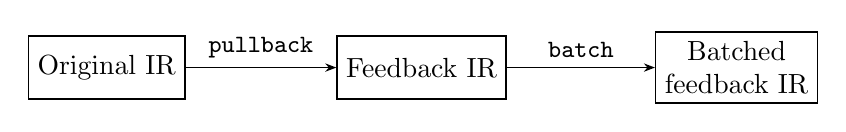
\begin{tikzpicture}[
    box/.style={draw, line width=0.5pt, minimum height=0.8cm,
                minimum width=1.8cm, align=center},
    flow/.style={-{Stealth[length=4pt]}, line width=0.5pt},
    note/.style={font=\small, align=center},
    choice/.style={diamond, draw, line width=0.5pt,
                   aspect=2, inner sep=2pt, align=center},
]

    \node[box] (ir) at (0,0) {Original IR};
    \node[box] (feedback) at (4,0) {Feedback IR};
    \node[box] (batch) at (8,0) {Batched\\feedback IR};
    \draw[flow] (ir) -- node[above,note] {\texttt{pullback}} (feedback);
    \draw[flow] (feedback) -- node[above,note] {\texttt{batch}} (batch);

\end{tikzpicture}
\end{document}
